\documentclass{article}

\usepackage[english]{babel}
\usepackage[letterpaper,top=2cm,bottom=2cm,left=3cm,right=3cm,marginparwidth=1.75cm]{geometry}

\usepackage{authblk}
\usepackage{amsmath}
\usepackage{graphicx}
\usepackage{natbib}
\usepackage{url}
% JK: turning this off for the moment as I keep clicking through on links
% to the bibliography while reading the text and it's intensely annoying.
% Can reinstate when we're ready to preprint
% \usepackage[hidelinks]{hyperref}

\usepackage{makecell}

\title{Towards a Pandemic-Scale Ancestral Recombination Graph of SARS-CoV-2}
\author[1]{Shing H. Zhan}
\author[2,5]{Katherine Eaton}
\author[3,5]{Anastasia Ignatieva}
\author[1,5]{Benjamin Jeffery}
\author[1,5]{Duncan S. Palmer}
\author[1,5]{Yan Wong}
\author[2]{Carmen L. Murall}
\author[4]{Sarah P. Otto}
\author[1,6]{Jerome Kelleher}
\affil[1]{Big Data Institute, Li Ka Shing Centre for Health Information and Discovery, University of Oxford, Oxford, United Kingdom}
\affil[2]{National Microbiology Laboratory, Public Health Agency of Canada, Canada}
\affil[3]{Department of Statistics, University of Oxford, Oxford, United Kingdom}
\affil[4]{Department of Zoology and Biodiversity Research Centre, University of British Columbia, Vancouver, British Columbia, Canada}
\affil[5]{Preliminary alphabetic ordering}
\affil[6]{Correspondence. E-mail: jerome.kelleher@bdi.ox.ac.uk}

\begin{document}
\maketitle

\begin{abstract}
XX
\end{abstract}

\section{Introduction}

Recombination via template switching is a common feature in the evolution of
coronaviruses (CoV) \citep{Graham2010-xe,De_Klerk2022-tt}), including SARS-CoV-2
\citep{VanInsberghe2021-eu,Jackson2021-ik,Ignatieva2021-rg}. By bringing
together mutations carried by different lineages, recombination plays an
important role in generating genomic diversity, with recombinant lineages
associated with CoV adaptation to new host species and with the production of
more immune evasive variants \citep{Graham2010-xe,De_Klerk2022-tt}.

Recombination was challenging to detect in SARS-CoV-2 early in the pandemic due
to gradual accumulation of genetic variation. In late 2020, the appearance and
spread of variants of concern (VoC) harbouring multiple characteristic
mutations increased the detectability of recombination. By searching for
genomes containing segments from different VoC, multiple recombinant lineages
have been detected, for example, between Alpha and pre-VoC
\citep{Jackson2021-ik}, Alpha and Epsilon \citep{Wertheim2022-hj}, and Alpha and
Delta \citep{Sekizuka2022-xz}). More recently, the high prevalence of Omicron,
with multiple co-circulating deeply divergent lineages (BA.1 to BA.5), has
accelerated the rate of coinfection and the potential for recombination
\citep{Bal2022-hq}. Recombinant lineages that have sufficient evidence of onward
transmission (more than five descendants) and monophyly (> 70\% bootstrap
support) are eligible for a Pango lineage designation \citep{Rambaut2020-dw},
starting with the letter X (“Pango Lineage Nomenclature: Provisional Rules for
Naming Recombinant Lineages” 2021).

Most genomic surveys for SARS-CoV-2 recombinants search for mosaic genomes that
combine specific subsets of mutations from different lineages (e.g.,
\citep{VanInsberghe2021-eu,Jackson2021-ik,Wertheim2022-hj,Sekizuka2022-xz}).
This approach only identifies those inter-lineage recombination events
resulting in the patterns investigated. Others have inferred recombinant
genealogies to disentangle recombination from recurrent mutation, without
having to pre-specify characteristic mutations for each lineage
\citep{Ignatieva2021-rg}. More recently, Turakhia et al. \citep{Turakhia2022-it}
has presented a phylogeny-based approach ("RIPPLES") to identify putative
recombinants among over ten million SARS-CoV-2 genomes, without pre-specifying
motifs. To find candidate recombinants, RIPPLES first builds a phylogeny
without assuming recombination and then scans for long branches (i.e., carrying
many mutations) and then determines if these candidates would be better
explained by recombination. Specifically, RIPPLES exhaustively breaks each
candidate sequence into segments and attempts to find more parsimonious
placements for each segment on the phylogeny. If such placements are found, the
sequence is identified as a putative recombinant. Although it enables rapid
searches for genomic evidence of recombinants, RIPPLES relies on a SARS-CoV-2
phylogeny that accounts for only mutations, treats recombinants \textit{post
hoc}, and is an incomplete representation of the reticulate evolutionary
history of SARS-CoV-2. As noted by the authors, a \textit{post hoc} treatment
of recombination is possible when recombinant lineages are rare and leave few
descendants, but this is becoming increasingly untenable with the proliferation
of recombinant lineages (e.g., more than half of the sequences sampled in
February, 2023 are from XBB and its descendants; \citep{Chen2022-pz}.

Inferring evolutionary trees while accounting for both mutation and
recombination is a long-standing challenge. This challenge is particularly
acute for SARS-CoV-2, given the large amount of data that has been shared, with
over 15 million sequences in the GISAID database \citep{Shu2017-hp}. It is well
known that recombination distorts phylogenies \citep{Schierup2000-fg} and
affects the results of downstream analysis (e.g., inference of selection;
\citep{Anisimova2003-vr}). However, standard phylogenetic methods do not account
for recombination (e.g., \citep{Ronquist2012-zw,Minh2020-lr,Guindon2003-zd}).
Alternatively, genetic ancestries of recombining lineages can be represented by
ancestral recombination graphs (ARG; \citep{Griffiths1981-lw,Hudson1983-if},
which  capture network-like phylogenetic relationships \citep{Gusfield2014-qw}.

Approaches to infer ARGs now exist that can scale to tens of thousands of human
genomes and beyond
\citep{Speidel2019-yh,Kelleher2019-ba,Zhang2021-lf,Schaefer2021-yg}. Recently,
Wohns et al. \citep{Wohns2022-th} reconstructed a unified whole-genome genealogy
of thousands of modern and ancient human genomes, based on over 90 million
variable sites. To achieve this, Wohns et al. \citep{Wohns2022-th} utilised
several computational advances in ARG inference: (1) the "succinct tree
sequence" data structure that can compactly store large ARGs
\citep{Kelleher2018-xc}; (2) a highly efficient Hidden Markov Model (HMM)
implementation of the Li and Stephens (LS) model (Li and Stephens 2003) to
infer copying paths between genomes \citep{Kelleher2019-ba}; and (3) efficient,
open-source software tools
\citep{Baumdicker2022-ep,Kelleher2018-xc,Kelleher2019-ba,Wohns2022-th}.

Here, we present a preliminary version of a novel scalable methodology
(“sc2ts”, pronounced “scoots”) that builds on the advances above and
additionally takes advantage of known collection dates to infer ARGs from
millions of full-length SARS-CoV-2 genomes. Using publicly available SARS-CoV-2
genome sequences, we demonstrate that sc2ts can be used to simultaneously (1)
detect putative SARS-CoV-2 recombinants; (2) infer the phylogenetic
relationships of the major SARS-CoV-2 lineages; (3) reconstruct the mutational
spectrum of SARS-CoV-2; and (4) provide a compact record of evolutionary
information about SARS-CoV-2 that can be efficiently accessed using "tskit"
(tree sequence toolkit) software library \citep{Kelleher2018-xc}. Sc2ts is a
promising method to automate detection of SARS-CoV-2 recombinants and to
jointly model recombinational and mutational processes shaping the genomic
diversity of SARS-CoV-2 at large scale.

\section{Methods}

\subsection{Data preprocessing}

\subsubsection{Sequence-level preprocessing}

The findings of this study are based on sequences and metadata available on
GISAID (\url{https://gisaid.org/}) up to Aug 22, 2022 and accessible at
doi.org/10.55876/gis8.230329cd (Supplementary Table 1). Sequences were removed
if they (1) had ambiguous collection dates; (2) were collected before January
01, 2020 or after June 30, 2022; or (3) were isolated from a non-human host.
Sequences were aligned to the Wuhan-Hu-1/2019 reference sequence (GenBank:
MN908947.3) using Nextclade v2.3.0 \citep{Aksamentov2021-hj} (dataset tag
2022-07-26T12:00:00Z). To reduce the impact of poor-quality sequences on ARG
inference, sequences were excluded if they had a “bad” quality control status
in any of the four Nextclade columns ("qc.missingData.status”,
“qc.mixedSites.status”, “qc.frameShifts.status”, and “qc.stopCodons.status”).
These excluded genomes are enriched for low-coverage, contaminated, or
misassembled sequences.

\subsubsection{Site-level preprocessing}

Ambiguous nucleotide letters (i.e., not A, C, G, T, or a gap) in the pairwise
genome alignments were encoded as N. Problematic bases in the alignments, which
had two or more ambiguous letters or gaps within a distance of seven bases,
were masked as missing data following the protocol in
\url{https://github.com/roblanf/sarscov2phylo/}. Masked bases were ignored
when attaching a sample genome to the ARG, but they were subsequently imputed.
Further, 481 problematic sites flagged as prone to sequencing errors or highly
homoplasic were excluded entirely
(\url{https://virological.org/t/issues-with-sars-cov-2-sequencing-data/473};
\url{https://raw.githubusercontent.com/W-L/ProblematicSites_SARS-CoV2/master/problematic_sites_sarsCov2.vcf}).

\subsubsection{Exclusion of “time travellers”}

Including samples with incorrectly reported collection dates (e.g., an Alpha
sample purportedly collected in 2020 from the United States, before Alpha
appeared in the United Kingdom, USA/MN-Mayo-1563/2020) was found to produce
artefacts that distorted the topology of ARGs inferred early on in the study.
Hence, to exclude such potential “time travellers”, we employed two filters.
The first was to remove any sequence with a collection date that pre-dated the
time to the most recent common ancestor (tMRCA) of its corresponding clade. The
tMRCA for each clade was obtained from a Nextstrain GISAID reference tree
(downloaded on August 22, 2022) where we used the lower bound of the 95\%
confidence interval of each clade as the minimum date cut-off. The second
filter was a simple threshold on the time delay between the collection date and
submission date (maximum submission delay, or MSD). Indeed, we found that ARGs
inferred from the MSD-filtered genome set had noticeably fewer branches with a
high number of reversions. After some preliminary analysis, a MSD threshold
value of 30 days was used when building the ARGs described herein. Future work
could estimate collection dates by adding these potential time travellers back
on the tree, allowing an automated assessment of collection date discrepancies.

\subsection{Inference}

\subsubsection{Overview of sc2ts}

We introduce an ARG inference method (schematic in Figure 1) that uses (1) an
efficient HMM implementation of the Li and Stephens (LS) model \citep{Li2003-ib}
to copy SARS-CoV-2 genomes (see Sections 2.2 and 2.3); (2) the reported
collection dates of the SARS-CoV-2 samples to determine the order of genome
copying; and (3) several parsimony-based heuristics to locally refine the
topology. In brief, this combined approach uses the likelihood model of LS to
attach sample genomes to existing nodes and to detect recombinants, but because
many of the tip samples attached daily harbour few, if any, mutational changes,
we use parsimony to resolve the relationships near the tip samples.

Our HMM implementation, sc2ts, builds a reticulated graph for SARS-CoV-2 by
taking advantage of the reported collection dates to incrementally grow the
ARG. The inference process occurs forward in time, attaching new genomes
aggregated by their collection date (daily batches), from the earliest to the
last collection date. Prior to attaching sample genomes, the ARG is initialised
such that the Wuhan-Hu-1/2019 reference genome is the root node. In the absence
of recombination, the ARG is a single tree with no reticulation (Figure 1A);
however, in the presence of recombination, a reticulate ARG is generated, with
variation in tree topology across the genome (Figure 1B). Unlike standard
phylogenetic trees in which internal nodes represent inferred ancestors,
internal nodes in the ARGs inferred using sc2ts represent ancestors which can
be samples or inferred ancestors.

Each daily batch of genomes is first attached to the growing ARG without any
phylogenetic resolution. In cases where the newly added sequence is inferred to
be a recombinant, a recombination node is inserted; the “date” of this node is
arbitrarily set to the average of the collection dates of the genome and the
most recent of its parent nodes. Otherwise, the genomes are attached to the
most closely related ancestral node (an attachment node). This creates
polytomies that are then locally resolved among the descendants of each
attachment node using the Unweighted Pair Group Method with Arithmetic Mean
(UPGMA) algorithm \citep{Michener1957-tr}, with average linkage (Figure 1C).
This hierarchical clustering algorithm produces a dendrogram relating a set of
sequences, which is treated as an ultrametric binary tree here. Subsequently,
mutations are placed onto the daily tree by maximum parsimony. An issue with
the UPGMA algorithm is that it may create internal nodes supported by no
informative site (i.e., having no mutation immediately ancestral to them). In
an adjustment step, such unsupported internal nodes are removed to “un-resolve”
the daily tree; the remaining internal nodes, which are supported by at least
one shared mutation, are retained. The “dates” of the non-sample internal nodes
are set to the same date as the samples in the daily batch. The resulting daily
tree is grafted onto the attachment node in the global ARG.

During ARG inference, two types of non-sample nodes are inserted to improve
parsimonious placement of mutations: mutation-coalescing nodes and
pushed-reversion nodes. We call these operations tree adjustments. A
mutation-collapsing node is inserted when a shared mutation between sibling
nodes is found (Figure 1D). An attempt to create mutation-collapsing nodes is
made after grafting a new daily tree onto the global ARG. If shared mutations
exist between two or more sibling nodes, then a parsimonious explanation is to
create a new node that is the parent of those siblings, on which these
mutations occurred. A pushed-reversion node is inserted when an immediate
reversion occurs (Figure 1E), i.e. a mutation that reverts another mutation on
its parent node. Instead of retaining both the mutation and immediate
reversion, only the mutation is kept after a pushed-reversion node is inserted,
thereby reducing the number of mutations on the branches. Note that these
non-sample nodes are used as reconstructed genomes during HMM copying.

Furthermore, during inference, the ARG is automatically encoded, stored, and
updated as a tree sequence using tskit \citep{Kelleher2018-xc}.

\subsubsection{Brief description of the Li and Stephens model}

The LS model is a convenient probabilistic approximation to the coalescent with
recombination \citep{Hudson1983-if}, itself a generative model of a genealogical
process with recombination \citep{Li2003-ib}. Importantly, it can be implemented
as an HMM in which a focal genome is a sequence of nucleotides (observed
states) that are probabilistically emitted as an imperfect mosaic of a set of
reference genomes (hidden states). As such, an efficient HMM machinery can be
employed to make statements about parameters of interest and highlight
potential sources of error in genotyping and sequencing data. The LS model is
used in a wide variety of applications in genomics. For example, it is the
engine that drives statistical genotype phasing and imputation
\citep{Delaneau2019-wl,Browning2021-cg,Browning2018-nk,Rubinacci2020-pa}, and it
can be used to estimate mutation rates (e.g., REF), recombination rates (e.g.,
\citep{Hinch2011-tz}), and selection within and across hosts in viral sequence
data (e.g., \citep{Palmer2019-wa}).

The generative process of the LS model is summarised in Figure 2. Here, a
transition matrix, Q, governs the process of switching (recombining) between
members of the reference panel (the hidden states). An emission matrix,
\textit{E}, allows for differences between the focal sequence and the hidden
state from which it is copied (due to mutation as well as genotyping or
sequencing error). Then, we use the Viterbi algorithm \citep{Viterbi1967-ol} to
find the most likely copying path through the sequences, given a set of
reference sequences, \textit{Q}, and \textit{E}.

Because the HMM is memoryless, the potential parental lineages are
independently assessed at each recombinantion breakpoint. This can result in
the inference of a recombinant lineage descending immediately from three (or
even more) parental lineages. We find that often two of the three parents are
identical or similar in sequence in the segments contributed to the recombinant
lineage. A more parsimonious explanation would be to switch back to the
original parent sequence. In the future, a pragmatic solution would be to
detect such cases during the ARG inference stage and to adjust the copying
paths accordingly. Meanwhile, however, we urge caution when interpreting the
parentage of lineages with multiple breakpoints.

\subsubsection{Parameterization of the HMM implementation of Li and Stephens
model}

Recombination is inferred using an efficient HMM implementation of the LS
model. Copying paths are estimated from SARS-CoV-2 genomes sampled over time,
with younger genomes copying (i.e. inheriting segments and mutations) from
older genomes. Here, we were able to apply the LS model on millions of
SARS-CoV-2 genomes because of a highly efficient, exact HMM implementation of
the LS model that is a core component of the tsinfer software. For this
application, we have parameterised the HMM using a mismatch ratio (MMR), which
tunes how strongly mutations (i.e., no switching of template sequences) are
preferred over recombination (i.e., switching between sequences) during
copying. Under a lower MMR value, the maximum-likelihood HMM copying path of a
focal genome more likely spans at least two ancestral genomes (i.e,. the focal
genome is a putative recombinant) than a single ancestral genome. Here, the MMR
was set to three in all the HMM runs (see Discussion for future potential
development of the HMM).

\subsection{Analysis}

\subsubsection{Imputation of Pango lineage for non-sample nodes}

Non-sample nodes inserted during ARG inference had no Pango lineage assignment
from Nextclade. We imputed the Pango lineage of non-sample nodes using a
two-step procedure (Figure 3) to help assess how consistently breakpoint
intervals are estimated by the HMM runs (see below). If the Pango lineage of
the parental node was available and no mutation was immediately ancestral to
the non-sample node, then the parental node’s status was directly propagated to
the non-sample node. Otherwise, the Pango lineage of the non-sample node was
inferred by matching its full set of mutations against the Pango
lineage-defining mutations (based on 90\% consensus of the sequences analysed)
from the COVID-CG website \citep{Chen2021-zc}; \url{https://covidcg.org/};
accessed on November 04, 2022).

\subsubsection{Breakpoint intervals and HMM consistency}

When recombinant ancestry for a given genome is inferred by the LS HMM, a
breakpoint is identified as the last possible position where the copying path
must switch. Thus, the breakpoints used in the ARG represent the rightmost end
of the interval, within which the recombination event could have occurred. To
obtain the leftmost end of this interval, we rerun the HMM using mirrored
coordinates (i.e., from the 3’ end to the 5’ end).

A recombinant sequence was deemed to be HMM-consistent if (1) the same number
of parent nodes and (2) the same set of mutations immediately ancestral to it
were obtained from both the unmirrored and mirrored HMM runs. In the ideal
case, the copying paths of both the HMM runs switch between parent sequences at
the same position(s); in less ideal cases, however, the copying paths switch at
different positions, typically because of a lack of genetic variation between
the positions. The switch positions in the copying paths of both the HMM runs
were used to define the breakpoint interval(s) of an HMM-consistent
recombinant.

\subsubsection{Code availability}

The source code implementing the sc2ts pipeline is available via GitHub
\url{https://github.com/jeromekelleher/sc2ts/}. The sc2ts pipeline uses
various functions and algorithms implemented in tskit and tsinfer
\url{https://github.com/tskit-dev/}. The pipeline uses the SciPy
implementation of the UPGMA algorithm to build daily trees
\url{https://docs.scipy.org/doc/scipy/reference/generated/scipy.cluster.hierarchy.average.html}.
The Jupyter notebooks used to produce the results described herein are also
available on GitHub \url{https://github.com/jeromekelleher/sc2ts-paper/}.

\section{Results}

\subsection{Inferred ARGs}

To illustrate the use of sc2ts, we employed two different sampling strategies.
First, we inferred a densely sampled but time-limited “wide” ARG by attaching
all the sample genomes with an MSD of 30 days, one daily batch at a time. The
inference procedure ran until the genomes sampled on June 30, 2021 were
attached to the ARG, resulting in a total of 1.27 million samples. Second, we
inferred a “long” ARG over a more extended timespan, by attaching at most 1,000
genomes, which were randomly subsampled from each daily batch with an MSD
within 30 days. For this ARG, the inference procedure ran until the genomes
sampled on June 30, 2022 were attached to the ARG. The long ARG covers an extra
year of samples but is more sparsely sampled. June 30, 2022 is the collection
date of the final batch of sequences which were preprocessed for the
development of sc2ts. Once sc2ts is further developed and tested, we will
attach samples collected after that date to infer a fully sampled
pandemic-scale ARG.

Most of the nodes in the ARGs represent sample genomes (Table 1). Only a small
fraction of the nodes represent recombination events (0.28\% and 0.27\% in the
wide ARG and long ARG, respectively), over half of which have no descendant
samples (besides the recombinant sequence that triggered insertion of the
recombination node) (Table 1). There are over one million mutations on the
ARGs, the majority of which occur on a terminal edge (Table 1). Notably, the
massive amount of genomic variation data in the wide ARG (1.27 million genomes)
and long ARG (657 thousand genomes) are compactly stored in ~57 Mb and ~36 Mb,
respectively (less than ten bytes per sample). These ARGs can be loaded for
analysis in a Jupyter notebook on a typical commercial laptop in merely a
fraction of a second using the Python package tskit (Table 1).

\subsection{Computational resources}

The wide ARG (with over one million sample genomes) was built using 128 threads
on a machine with 512 GB RAM (2x AMD EPYC 7502 @ 2.5GHz). Inference ran for 17
days to attach genomes sampled up to June 30, 2021. The long ARG (with ~700
thousand sample genomes) was built using 40 threads on a machine with 256 GB
RAM (2x Intel(R) Xeon(R) CPU E5-2680 v2 @ 2.80GHz). Inference ran for 23 days
to attach genomes sampled up to June 30, 2022. Most of the runtime was spent on
running the HMM.

\subsection{Backbone phylogeny}

For validation purposes, we compare the genetic relationships in the
sc2ts-inferred ARGs with phylogenetic relationships inferred by the NextStrain
project \citep{Hadfield2018-ef}. The NextStrain trees consist of subsamples of
SARS-CoV-2 genomes, which over the time period of our ARGs are almost entirely
restricted to non-recombinant lineages. To allow for comparison, the ARGs were
"simplified" \citep{Kelleher2018-xc} to retain only those tips of our genealogy
that match the samples present in a specific NextStrain tree. These simplified
"backbone" ARGs exhibit very little recombination (6 and 5 trees across the
genome for the wide and long ARGs, respectively).

Figure 4 shows a co-phylogeny of the 88 samples shared between the wide ARG and
a GISAID global "all-time" tree from NextStrain (downloaded on January 21,
2023). To reduce the ARG to a single tree, we show the very first tree in the
wide ARG; however, the five other trees in this simplified ARG show
near-identical patterns. Supplementary Figure 3 shows the same comparison for
the long ARG. It is clear that the backbone topology of the sc2ts tree shows
very close agreement with the NextStrain tree. The sample genomes cluster by
their assigned Pango lineage status, and many variants and their descendents
form identical monophyletic clades in both the trees (e.g., the Alpha and Delta
clades).

There are, however, some notable differences between the trees. Firstly, the
sc2ts tree is generally less well resolved (noticeably, February to March,
2020) (Figure 4). Secondly, there are non-identical sample partitions near the
tips (e.g., in the Alpha clade, Figure 4). These might have arisen because the
samples containing the mutations needed to resolve local topologies were
collected later than the cut-off date for the sc2ts ARG, but were for the
NextStrain tree. Finally, the branch lengths differ. For example, the branch
leading to the ancestral node of the Delta variant samples is much shorter in
the sc2ts tree than the NextStrain tree (Figure 4). It is possible that the
length of some of the branches was poorly calibrated, probably caused by overly
aggressive insertion of mutation-collapsing nodes and reversion-pushed nodes or
suboptimal sample attachment. Side-by-side comparison of sc2ts trees with trees
inferred using another method (e.g., UShER) should help to understand whether
branch length differences are due to poor calibration or methodological
differences.

Although here we focus on a single local tree at an arbitrarily chosen
position, note that in the original “un-simplified” ARGs, there are 1,496 and
958 trees, respectively (Table 1). Hence, while for a relatively small sample
the genealogy may be well described by a single tree, the full dataset shows
substantial variation in phylogenetic relationships (or phylogenetic
incongruence) across the SARS-CoV-2 genome, much of which may be attributable
to recombination. Such complex reticulate relationships are appropriately
captured by a genealogy in the form of an ARG.

\subsection{Putative recombination events}

Both the wide and long ARGs contain a large number of recombination nodes
(4,123 and 2,078, respectively; Supplementary Tables 1 and 2), with each of
these nodes inferred as a result of matching a specific sample (a recombinant)
into the ARG. However, ~65\% of recombination nodes are ancestors of only a
single descendant sample in each local tree; these could have arisen from
sequencing of mixed samples (e.g., from co-infection or contamination), or were
simply not transmitted onwards and so were excluded from subsequent analyses
(leaving X and Y recombinants in the wide and long ARGs, respectively). In
their analysis using RIPPLES, Turakhia et al. (2022) detected 589 recombinants,
also excluding singletons.

For simplicity, we focus primarily on “non-complex” recombination nodes. To do
this, we apply a filtering step that removes those with more than one
breakpoint (and often more than two parent lineages), or where matching is not
HMM-consistent or identifies parents with different Pango lineage assignments
in the original (i.e., 5’ to 3’ end) and mirrored (i.e., 3’ to 5’ end) HMM
runs. Filtering reduces both the number of recombination nodes and breakpoints
from  A \& B to C in the wide ARG and from 726 \& 806 to 459 in the long ARG
(Supplementary Tables 1 and 2). Note that in the unfiltered case, a single
recombination node can correspond to multiple points, one for each
recombination breakpoint. The effect of this filtering step in the long ARG,
which includes time periods of increased rates of coinfection and recombination
compared to the wide ARG, can be seen in Figure 3A (unfiltered) and Figure 3B
(filtered).

Importantly, the long ARG captured all except one of the Pango designated
recombinant lineages (see the section below), but we also detected a large
number of additional recombination events, with parents lineages that diverged
as far back as two years to as recent as five or six days prior to the
recombination event (Figure 3). This provides a degree of resolution of viral
recombinants not available with other recombination detection methods. The
majority of newly identified recombinants arise from parents that diverged 10
to 30 weeks previously. However, there is also a peak of recombinants that
diverged ~95 weeks prior to the event: these correspond to recombinants whose
parental common ancestor traces to early 2020, including both Delta-Delta and
Delta-Omicron recombinants (Supplementary Figure 4).

The date of common ancestry for the two parents of recombinant lineages is
concentrated in several banded rows in Figure 5. These are largely due to a
small handful of most recent common ancestors (MRCAs), which are shared between
a large number of recombination events, the top four of which are indicated by
dotted lines in the figure. These MRCAs are near the root of large expansions
of certain lineages (B.1: original variant;  B.1.617.2: Delta, BA.1: first
Omicron wave; and BA.2: second Omicron wave), as evidenced by the number of
samples with that Pango designation that trace back to these ancestral nodes
(listed as percentages on the plot). The specific MRCA nodes to which many
recombinants trace frequently represent very large polytomies in the tree (at
the extreme, 2,872 immediate children). This is likely to indicate a rapid and
under-sampled expansion of a clade in the SARS-CoV-2 genealogy.

Finally, it is clear from Supplementary Figure 4 that of the recombinant
parents that can be classified into Alpha, Delta, and Omicron variants, the
majority are within-Delta and within-Omicron recombinants, and that Omicron
followed by Delta, are the variants associated with the most recombination.
This may reflect either sampling intensity, the prevalence of cases (which
increases the chance of coinfection and recombination), or possibly
heterogeneity in recombination rates among lineages.

\subsection{Early recombinants reported by Jackson et al. (2021)}

By searching for samples combining genomic segments from Alpha (B.1.1.7) and
from the parental lineage B.1.1 based on a list of 22 Alpha-defining mutations,
Jackson et al. (Jackson et al. 2021) reported 16 recombinant sequences among
genomes sampled in the United Kingdom up to March 7, 2021. The authors proposed
that the recombinants likely arose from eight independent recombination events
(categorised into groups A to D and four singletons).

In the wide ARG (sampled to mid-2021), all these sequences are descendants of
recombination nodes, except MILK-103C712, which was removed during
preprocessing (Table 2); additionally, all are HMM-consistent, except
QEUH-1067DEF. Overall, we find excellent agreement between Jackson et al.’s
motif-based method and sc2ts in terms of (1) the Pango lineage of the parents
and (2) the breakpoint intervals (Table 2). In all cases, the two methods
proposed identical or very closely related parent lineages. The general mosaic
genome structure is concordant in all the cases, even CAMC-CB7AB3 where there
are two switches in the HMM copying paths (indicative of two breakpoints). The
breakpoint intervals estimated using the two methods overlap substantially in
all the cases (Table 2). Within each of the groups A to D, the constituent
sequences have identical breakpoint intervals, because they trace back to a
single recombination node in the wide ARG. This result is consistent with the
hypothesis that the sequences of the groups A to D emerged from four separate
recombination events (Jackson et al. 2021).

\subsection{Pango recombinants}

The wide ARG only contains samples from three Pango-designated recombinant
lineages (XA, XB, and XC), due to the fact that it only includes samples up to
mid-2021. By contrast, the long ARG (subsampled to mid-2022) contains samples
from 33 Pango-designated recombinant lineages (XA to XAK; Supplementary Table
3). For Pango recombinant analysis, we therefore focus on the long ARG.

In the wide ARG, every sequence of the three Pango recombinants trace back to
some recombination node. XA, XB, and XC.

In the unfiltered long ARG, the sequences of 28 Pango recombinants trace back
to some recombinant node(s); however, the sequences of the five Pango
recombinants XP, XU, XAA, XAG, and XAK do not. A likely explanation for the XP
recombinant sequences not having a recombinant origin in the long ARG is that
its characteristic multibase deletion
(https://github.com/cov-lineages/pango-designation/issues/481) was masked
during preprocessing and therefore was not incorporated into the HMM. Upon
tracing the origin of XAG through the ARG, XAG might have been caused by
incorrect imputation of its parent nodes(?). XAK likely does not appear to have
a recombinant origin because of random subsampling, but it may with a more
complete tree.

The sequences of 14 Pango recombinants trace back to a single recombination
node. The sequences of the remaining 18 Pango recombinants trace back to
multiple recombination nodes, however. This may be a result of undersampling in
the long ARG, which was built by randomly subsampling at most 1,000 sequences
from each daily batch. Having extra recombination nodes in the long ARG
appeared to be a more parsimonious explanation for the 19 Pango recombinants
than having a single recombination node with many immediately ancestral
mutations (including recurrent mutations and reversions), despite that the
recombinants may indeed trace to a single origin.

The mosaic genome structure of all the 32 Pango recombinants is concordant with
the structure determined by the Pango Lineage Designation Committee
(Supplementary Table 3). For example, the genome of XD (also known as
“Deltacron”) is inferred to consist of B.1.617.2 (Delta) on the 5’ end, BA.1.17
(Omicron) in the middle, and B.1.617.2 (Delta) on the 3’ end.

\subsection{Novel recombinants}

Next, we examine recombination nodes in the filtered long ARG (sampled to
mid-2022) that represent previously unnamed putative recombinant sequences,
which do not have a Pango recombinant designation. For this proof-of-concept
study, we have arbitrarily picked 12 recombination nodes that seem plausible
(Supplementary Table 4). Coincidentally, all these nodes involve Omicron
subvariants (BA.1, BA.2, BA.4, and BA.5). These recombination nodes (1) were
inserted into the long ARG on or after January 8, 2022; (2) have at least 10
descendent samples; and (3) have no mutational differences (including immediate
reversions) from their parent nodes.

TODO: Node  740761 (USA/NC-CDC-LC0668306/2022) is a sister clade proposed1006
in the UShER public phylogeny. Node 628656 (Scotland/QEUH-37794BB/2022) is a
sister clade of XAC, and annotated as “miscBA2BA1PostSpike”.

\subsection{Recombinant origins of the Pango lineages XA and XAG}

XX

\subsection{Distribution of recombination breakpoint intervals}

We explore recombination signals across the SARS-CoV-2 genome by inspecting the
breakpoint intervals of the filtered recombination nodes from the wide ARG
(sampled to mid-2021) (Figure 4). The length of a breakpoint interval reflects
uncertainty in the estimated location of a breakpoint. On average, the length
of the breakpoint intervals is 2,895 bases (median, 1,670 bases; range, 1 to
23,666 bases). This broad distribution of interval length indicates that the
location of a breakpoint often could not be precisely determined given the
observed genetic variation.

There is a preponderance of breakpoint intervals spanning the 3’ end of the
genome (Figure 4A), as noted previously by Turakhia et al.
\citep{Turakhia2022-it}. Inspecting more closely, we find an enrichment in the
number of intersecting intervals in the E gene, ORF8, ORF8-N intergenic region,
and 3’ untranslated region (Figure 4B). Markedly, there is an abrupt drop in
the number of intersecting intervals in the N gene following the peak in ORF8
towards the 3’ end.

Next, we investigate the potential recombination signals alongside the number
of mutations across the genome (Figure 4C). Regions with a higher density of
mutations contain more genetic variation, increasing the power to detect
recombination events. The position 28,271 (located in the ORF8-N intergenic
region) has a particularly high number of mutations in the samples (Figure 5).
At this position, mutations (n = 7,572), insertions (n = 5,782), and deletions
(n = 1,605) appear to occur frequently. One possible explanation is that this
homopolymeric region is prone to sequencing errors, giving rise to an
artifactual recombination signal. At the upstream position 27,972, numerous
mutations also occur. This position has been reported to be hypermutable
\citep{Jungreis2021-dh}.

We further consider the breakpoint intervals within the context of
recombination breakpoint sequence motifs. It is hypothesised that certain
palindromic breakpoint sequences (specifically, CAGAC and CAGAT) promote
template switching during replication in SARS-CoV-2 via formation of
base-paired stem loops in the genome structure \citep{Gallaher2020-lb}. There
are 87 occurrences of these two breakpoint sequences in the Wuhan-Hu-1/2019
reference sequence (Supplementary Table 5). We observe that XX (XX\%) of the
breakpoint intervals of the HMM-consistent recombinants span at least one of
the breakpoint sequences.

\subsection{Mutational spectrum}

In addition to recombination events, the ARGs record mutation events along the
SARS-CoV-2 phylogeny. Yi et al. \citep{Yi2021-sc} reconstructed a SARS-CoV-2
phylogeny of over 350,000 genomes sampled globally from December 24, 2019, to
January 12, 2021, and systematically catalogued all the mutations occurring
along the phylogeny. Notably, in the mutational spectrum described by Yi et
al., C-to-U and G-to-U mutations occur more frequently than U-to-C and U-to-G
mutations, respectively.

For validation purposes, we compare the mutational spectrum from the wide ARG
with the mutational spectrum of Yi et al. We categorised all of the single
nucleotide mutations by type (defined by the ancestral state and derived
state), excluded mutations inherited by only a single sample (which are
enriched for sequencing errors and artefacts), and tallied them up by type.
Similarly, we took the data for single nucleotide mutations from Yi et al.
\url{https://github.com/ju-lab/SC2_evol_signature}, excluded mutations
occurring along terminal branches, and tallied them up by type. We find that
the mutational spectrum from the wide ARG (448,825 mutations) matches the
mutational spectrum reported by Yi et al. (92,344 mutations) (Figure X). In
both spectra, C-to-U mutations and G-to-U mutations occur more frequently than
U-to-C and U-to-G, respectively (Figure X). Similar results are obtained when
including the mutations inherited by only a single sample or occurring on
terminal branches (data not shown).

\subsection{Mutations under selection}

XX

\section{Discussion}

The COVID-19 pandemic continues to be a global emergency, with persistent high
levels of infection. This high prevalence has allowed the proliferation of many
variants, with more than 600 Pango-designated lineages circulating globally in
the last three months (January to March, 2023; https://gisaid.org/; access on
March 27, 2023). High prevalence also brings a higher risk of coinfection,
increasing opportunities for new phenotypically distinct recombinants to emerge
and spread.

In this proof-of-concept study, we demonstrate the feasibility of
reconstructing a large ARG from over one million SARS-CoV-2 genomes, a feat
that is simply not possible using other available ARG inference methods
(Rasmussen et al. 2014; Ignatieva et al. 2021; Speidel et al. 2019). We have
accomplished this feat by building on top of recent advances in storing and
processing large ARGs (tskit) and inferring genealogical relationships
efficiently at scale (tsinfer). The highly compact representation of the ARGs
as succinct tree sequences, coupled with vectorised computing technologies,
enables the large SARS-CoV-2 ARGs to be loaded in less than one second in a
Jupyter notebook and allows for each SARS-CoV-2 genome to be stored in less
than eleven bytes of data. We believe that further development of the sc2ts
methodology and software can create a powerful tool (1) to efficiently detect
emerging or previously overlooked recombinants in SARS-CoV-2; (2) to jointly
model the mutational and recombinational processes shaping global SARS-CoV-2
genomic diversity; and (3) to perform a broad variety of evolutionary analyses
of SARS-CoV-2 genomes with unprecedented global sequencing coverage.

ARGs are rich genealogical structures that contain information about the
genetic relationships among sampled genomes in the presence of recombination.
Here, we have conducted several analyses of the preliminary ARGs to show that
the ARGs built using sc2ts can (1) recapitulate the phylogenetic relationships
among major SARS-CoV-2 lineages; (2) recover biologically plausible
recombination signals in SARS-CoV-2 genomes; and (3) model mutation events in
SARS-CoV-2 evolutionary history.

ARGs reconstructed using sc2ts capture the phylogenetic relationships of major
SARS-CoV-2 lineages. Our results show that the backbone topology of a densely
sampled wide ARG inferred using sc2ts agrees well with the backbone topology of
a NextStrain tree inferred using IQ-Tree2, a widely used phylogenetic inference
package. However, we have noted several areas of differences (e.g., poorly
calibrated branch lengths), which are the focus of future development of sc2ts.
We believe that some of these differences can be reduced by improving and
refining our approach and strategy to handle samples with erroneously reported
collection dates (i.e., time travellers that have passed the maximum submission
delay of 30 days) and to modify the topology of daily trees.

Our results show that sc2ts identifies the early recombinants (pre-2022)
previously identified by Jackson et al. (2021). Sc2ts also identifies many
Pango recombinants, which are designated after community perusal of supporting
genomic evidence. We have found several previously unreported and overlooked
recombinant sequences in the wide ARG. After further improvements and
enhancements, we will use sc2ts to build a comprehensive ARG to search for
recombination signals among all the 15 million and counting SARS-CoV-2 genomes
available.

“The rate of putative recombination breakpoints is about three times higher
towards the 3' of the change point than the 5' interval.“ Consistent with this,
the breakpoint intervals of the putative recombinants identified here tend to
occur on the 3’ end of the SARS-CoV-2 genome.

\section{Improvements}

Currently, sc2ts is in development. Below, we propose several ways to
potentially improve or enhance sc2ts. We welcome suggestions and ideas from
experts.

\begin{itemize} \item A potential source of error in sc2ts ARGs comes from
incorrectly reported collection dates of the samples, which can cause sample
genomes to be attached to the wrong parts of the ARGs. Thus far, we have
attempted to correct the most offending errors in the ARGs by filtering out
"time travellers", but the sampling time can still be wrong by days or tens of
days. ***describe possible approaches to correct this?*** \item To avoid time
travellers, we used a maximum submission delay, but this will systematically
bias against submissions from countries with greater submission delays (Kalia
et al.). An area of future work is to add back the excluded sequences to a
built ARG to assess which ones are likely true time travellers. \item To avoid
time travellers, we used a maximum submission delay, but this will
systematically bias against submissions from countries with greater submission
delays (Kalia et al.). An area of future work is to add back the excluded
sequences to a built ARG to assess which ones are likely true time travellers.
\item We have used a single mismatch value in all the HMM runs, set so that
having three mutations is as likely as having a single recombination. This
parameter choice is arbitrary, and higher values may reduce the number of
origins for those Pango lineages that were inferred to descend from more than
one recombinant ancestor. In addition, because both the mutation rate and
recombination rate varies across the SARS-CoV-2 genome, it may be helpful to
allow the mismatch value to vary along the genome. \item By treating mutations
equally in the current HMM implementation, we implicitly assume that the rates
of different types of mutations are identical. However, as reported previously
(Yi et al. 2021), there is a high degree of mutational asymmetry in SARS-CoV-2.
To account for mutational biases, more sophisticated nucleotide substitution
models (e.g., allowing for different rates of transition and transversion) can
be incorporated into HMM likelihood calculations. \item Our current masking
strategy handles indels as missing data. Doing this can remove information
helpful to detect recombinants. For example, sequences of the Pango recombinant
XP were not identified as recombinants, because XP’s characteristic multibase
deletion was masked. \item This "lack of memory" in the HMM can create
recombinants with three or more parents when it would be equally parsimonious
to have just two. The copying process in the HMM currently does not limit the
number of parents to two, but doing so would be a valuable addition. \item Some
recombinants may reasonably have three or more parents, indicating multiple
"stacked" recombination events. We have largely ignored these in the current
analysis, but with further sc2ts development, there is potential to analyse
these putative recombinants and trace their evolutionary origins through the
ARG. \item In the present implementation, HMM traceback is performed once,
yielding a single maximum-likelihood genome copying path. A stochastic
traceback algorithm (e.g., (Rasmussen et al. 2014)) can be implemented in order
to quantify uncertainty about putative parent node(s) and switch positions.
These estimates of uncertainty may be used as support values for branches
analogous to bootstrap values produced by standard phylogenetic methods. \item
Daily trees are built using the UPGMA algorithm. This entails an extra step to
“un-resolve” daily trees in parts of the trees with no phylogenetic resolution.
To avoid this step, a better approach is to use a maximum-parsimony algorithm
to build daily trees instead. \end{itemize}

\section{Conclusions}

The global understanding of viral evolution during the COVID-19 pandemic is
unprecedented, with over 15 million sequences shared to date. We envisage that
once fully developed and tested, sc2ts methodology and software may provide a
unified computational framework to study the evolution and epidemiology of
SARS-CoV-2 at pandemic scale. The evolutionary analyses presented herein
exemplify the numerous applications possible using the ancestral recombination
graph inferred by sc2ts. We invite bioinformaticians, evolutionary biologists,
and virologists to join us and the broader tskit community to build the most
complete representation of the evolutionary history of SARS-CoV-2. Moreover,
while we have focussed on the particular application to SARS-CoV-2, the methods
we describe are readily applicable to the analysis of many other viral
pathogens. Solving the challenges in building and analysing large viral
genealogies would therefore contribute to the important goal of improving
preparedness for potential future pandemics.

\section{Acknowledgements}

We gratefully acknowledge all data contributors, i.e., the Authors and their
Originating laboratories responsible for obtaining the specimens, and their
Submitting laboratories for generating the genetic sequence and metadata and
sharing via the GISAID Initiative, on which this research is based. Also, we
thank Dr. Morag Graham (the National Microbiology Laboratory, Winnipeg, Canada)
for kindly providing the genomic coordinates of the breakpoint sequence motifs.
SHZ is supported by the Janssen-Oxford Translational Genomics Fellowship. JK,
YW, and BJ are supported by the Robertson Foundation.

\begin{table} \centering \begin{tabular}{l|l|l} \hline \textbf{Property} &
\textbf{Wide ARG} & \textbf{Long ARG} \\ \hline Last sampling date & 2021-06-30
& 2022-06-30 \\ Local trees & 1,496 & 958 \\ \hline
\multicolumn{3}{l}{\textit{Nodes}} \\ All nodes (sample and non-sample) &
1,453,347 & 783,231 \\ Sample nodes & 1,265,685 (87\%) & 657,239 (84\%) \\ Tree
adjustment nodes (excluding recombination nodes) & 80,830 (6.34\%) & 72,107
(10.97\%) \\ Recombination nodes & 4,123 (0.28\%) & 2,078 (0.27\%) \\ \hline
\multicolumn{3}{l}{\textit{Types of recombination nodes}} \\ Singletons (i.e.
no descendant besides the sequence causing insertion of the node) & 2,601
(63\%) & 1,315 (63\%) \\ Two-parent recombinants & 3,521 (85\%) & 1,869 (90\%)
\\ HMM-consistent recombinants & XX (XX\%) & XX (XX\%) \\ \hline
\multicolumn{3}{l}{\textit{Mutations}} \\ Total mutations & 1,213,193 &
1,062,072 \\ Mutations on a terminal edge & 758,903 (62.55\%) & 767,111
(72.23\%) \\ Recurrent mutations & 74,719 (6.16\%) & 50,099 (4.72\%) \\
Reversions & 72,617 (5.99\%) & 48,226 (4.54\%) \\ Immediate reversions (one
intervening node only) & 3,541 (0.29\%) & 1,347 (0.13\%) \\ \hline
\multicolumn{3}{l}{\textit{Storage and loading time}} \\ tszipped file
(including sample metadata, imputed Pango lineage assignments, and results of
HMM runs for recombination nodes) & ~57 Mb & ~36 Mb \\ Bytes to encode one
sample & 8.29 & 10.83 \\ Load time (seconds) & 0.9 & 0.5 \\ \hline
\end{tabular} \end{table}

\begin{table} \centering \begin{tabular}{l|c|c|c|c|c} \hline
\multicolumn{1}{c}{} & \multicolumn{3}{c}{\textbf{Jackson et al. (2021)}} &
\multicolumn{2}{c}{\textbf{sc2ts (wide ARG)}} \\ \hline \textbf{Sample} &
\textbf{Group} & \textbf{Parents} & \thead{Breakpoint \\ interval(s)} &
\textbf{Parents} & \thead{Breakpoint \\ interval(s)} \\ \hline ALDP-11CF93B & A
& \thead{B.1.177 \\ Alpha} & 21,255–21,613 & \thead{B.1.177.18 \\ Alpha} &
21,256–22,227 \\ ALDP-125C4D7 & A & \thead{B.1.177 \\ Alpha} & 21,255–21,613 &
\thead{B.1.177.18 \\ Alpha} & 21,256–22,227 \\ ALDP-130BB95 & A &
\thead{B.1.177 \\ Alpha} & 21,255–21,613 & \thead{B.1.177.18 \\ Alpha} &
21,256–22,227 \\ LIVE-DFCFFE & A & \thead{B.1.177 \\ Alpha} & 18,998–20,294 &
\thead{B.1.177.18 \\ Alpha} & 21,256–22,227 \\ QEUH-CCCB30 & B &
\thead{B.1.36.28 \\ Alpha} & 6,528–6,953 & \thead{B.1.36 \\ Alpha} &
6,529–6,954 \\ QEUH-CD0F1F & B & \thead{B.1.36.28 \\ Alpha} & 6,528–6,953 &
\thead{B.1.36 \\ Alpha} & 6,529–6,954 \\ MILK-1166F52 & C & \thead{Alpha \\
B.1.221.1} & 25,996–27,441 & \thead{Alpha \\ B.1.221} & 25,997–27,972 \\
MILK-11C95A6 & C & \thead{Alpha \\ B.1.221.1} & 25,996–27,441 & \thead{Alpha \\
B.1.221} & 25,997–27,972 \\ QEUH-109B25C & C & \thead{Alpha \\ B.1.221.1} &
25,996–27,441 & \thead{Alpha \\ B.1.221} & 25,997–27,972 \\ MILK-126FE1F & D &
\thead{B.1.36.39 \\ Alpha} & 20,703–23,062 & \thead{B.1.36.39 \\ Alpha} &
22,445–23,063 \\ RAND-12671E1 & D & \thead{B.1.36.39 \\ Alpha} & 20,703–23,062
& \thead{B.1.36.39 \\ Alpha} & 22,445–23,063 \\ RAND-128FA33 & D &
\thead{B.1.36.39 \\ Alpha} & 20,703–23,062 & \thead{B.1.36.39 \\ Alpha} &
22,445–23,063 \\ CAMC-CBA018 & n/a & \thead{B.1.177 \\ Alpha} & 20,389–21,254 &
\thead{B.1.177 \\ Alpha} & 16,177–21,255 \\ CAMC-CB7AB3 & n/a & \thead{Alpha \\
B.1.177 \\ Alpha} & \thead{3,267–4,474 \\ 20,389–21,254} & \thead{Alpha \\
B.1.177 \\ Alpha} & \thead{3,268–5,388 \\ 16,177–21,255} \\ MILK-103C712 & n/a
& \thead{B.1.177.17 \\ Alpha} & \thead{408–444 \\ 26,801–27,876} & n/a & n/a \\
QEUH-1067DEF & n/a & \thead{Alpha \\ B.1.177.9} & 10,523–10,869 & \thead{Alpha
\\ B.1.177} & 7,729–10,870 \\ \hline \end{tabular}
\caption{\label{tab:jackson}Recombinant sequences involving the Alpha (B.1.1.7)
variant reported by Jackson et al. \citep{Jackson2021-ik} have recombinant
ancestry in the wide ARG. The breakpoint intervals and Pango lineage
assignments of the parents were taken from Table 2 (3SEQ results) of Jackson et
al., except the Pango lineage assignment of the parents of group B
recombinants, which were taken from Table 1 (motif-based results).} \end{table}

\begin{figure} \centering
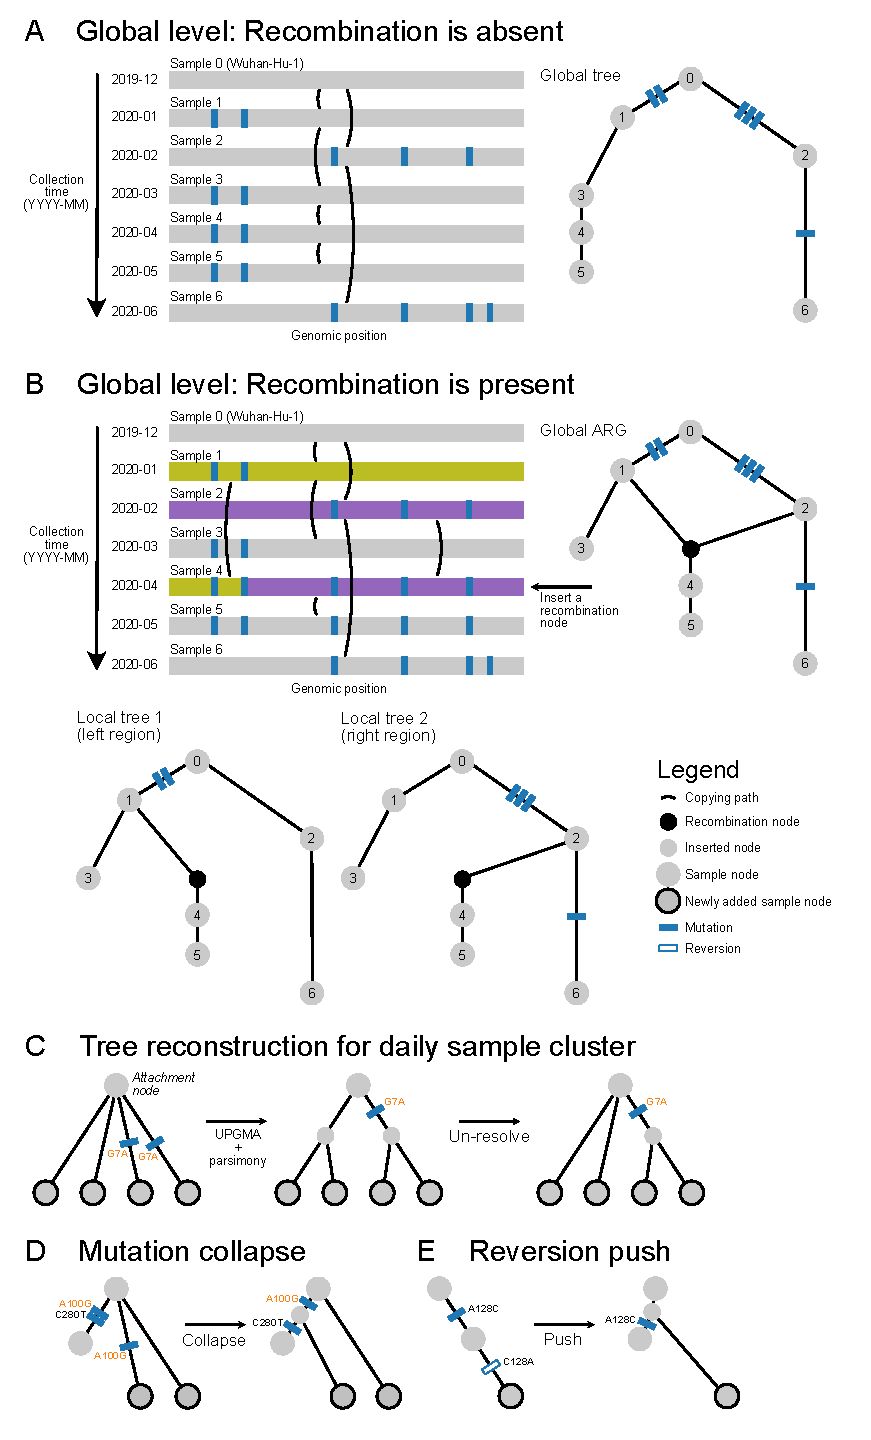
\includegraphics[width=0.7\textwidth]{figures/overview_sc2ts.pdf}
\caption{\label{fig:overview_sc2ts} A schematic of the sc2ts method. Sc2ts
reconstructs the genetic relationships among SARS-CoV-2 genomes by copying
samples to all possible ancestors collected at earlier time points (curved
arrows). An ARG is built by attaching new sample genomes grouped by collection
date to an existing ARG rooted at the Wuhan-Hu-1 reference genome, day by day.
Each iteration involves three stages: (1) attachment of new samples to the
growing ARG (A, B); (2) reconstruction of trees relating the samples under each
attachment node (C); and parsimony-based tree topology adjustments (D, E). In
the absence of  recombination, sc2ts infers an ARG that is a single tree
relating the samples (A). However, in the presence of recombination, sc2ts
infers an ARG that is encoded as a sequence of local trees relating segments of
the sample genomes (B), inserting a recombination node to represent a putative
recombination event. Additionally, mutation-collapsing nodes (D) and
pushed-reversion nodes (E) are inserted to make more parsimonious placements of
mutations that should be shared or should not be immediately reverted,
respectively.} \end{figure}

\begin{figure} \centering
\includegraphics[width=0.8\textwidth]{figures/ls_diagram_covid.pdf}
\caption{\label{fig:ls_diagram} A schematic of the Li and Stephens (LS) model.
The LS model in its implementation as an HMM is governed by the transition and
emission matrices, \textit{Q} and \textit{E}, respectively. Each may be a
function of the reference panel members, but transitions are generally assumed
to be independent of the hidden states themselves (shown in the pink panel).
This dramatically increases performance as the state space drops to two states
(i.e., switching or not switching). The recombination probability at site
\textit{l} is \textit{rl}, while n denotes the number of members in the
reference panel. Emissions may also be a function of the nucleotide states, but
in our case, we assume that all observed alleles (in both the reference panel
and focal sequence, \textit{al}) at the site under consideration are equally
likely and occur with mutation probability \textit{l} (shown in the blue
panel). These two processes, transition and emission (which encode
recombination and mutation, respectively), define the generative process of the
HMM, by which an imperfect mosaic is emitted from a reference panel of samples
and nodes from the ARG inserted at earlier collection dates (shown in the lower
panel). Here, the unseen states in the reference panel are shown as coloured
lines enclosed by the grey box, and the true path through the data which leads
to the emitted focal sequence is displayed by the black arrow. Examples of
transition and emission probabilities along this trajectory are shown by the
red and blue arrows, respectively. Black crosses along the focal sequence show
genotyping errors or mutations. Note that in practice, we do not know the
pattern of colours along the focal sequence and must infer it using the Viterbi
algorithm.} \end{figure}

\begin{figure} \centering
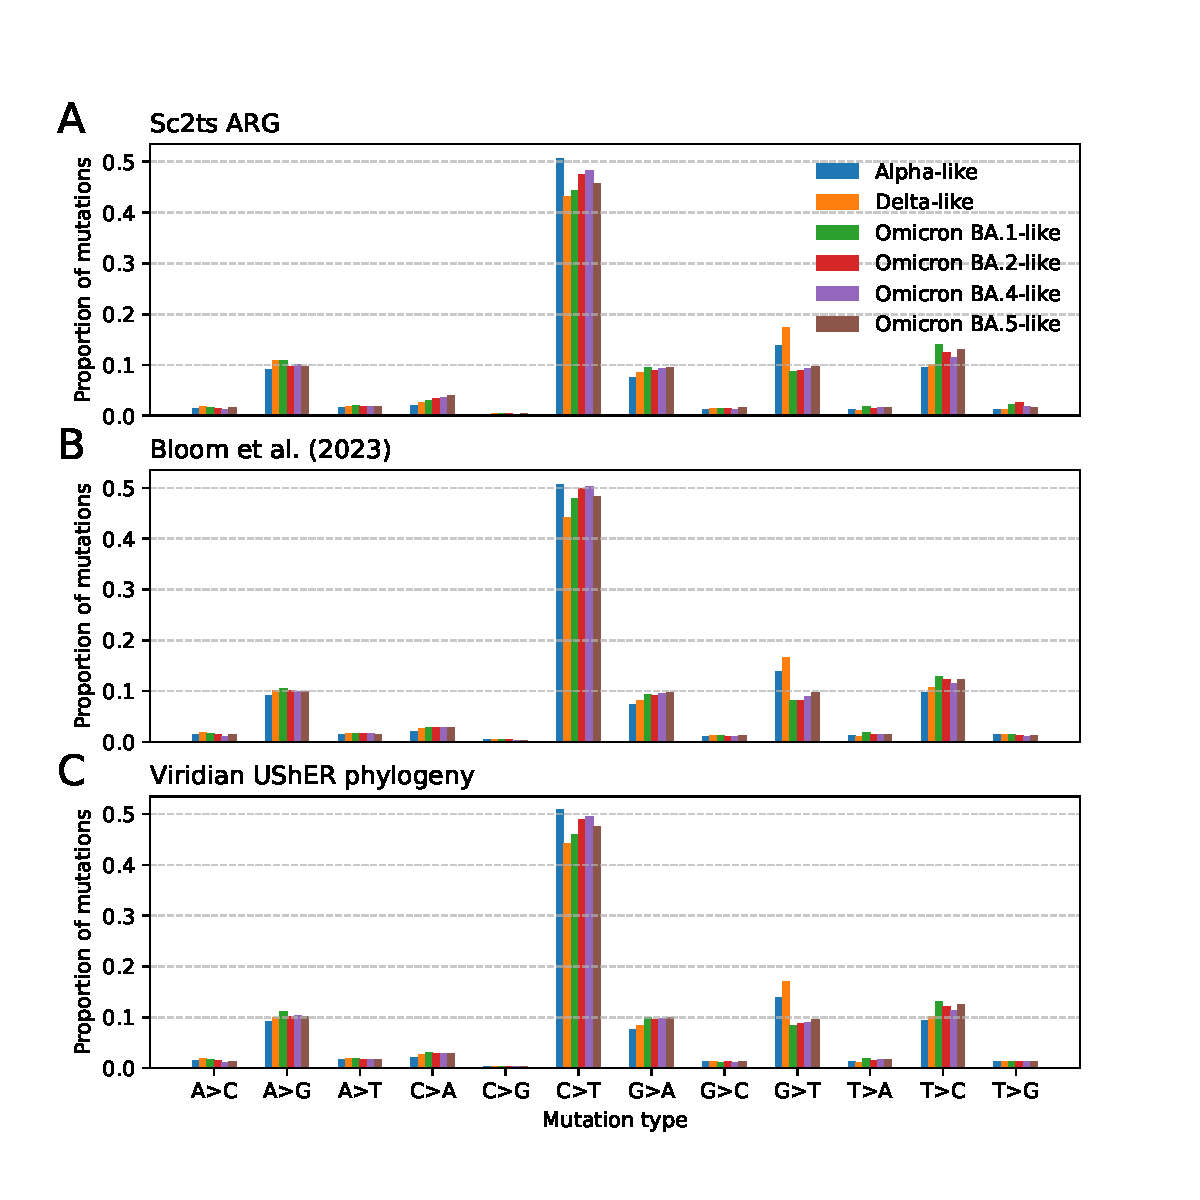
\includegraphics[width=0.8\textwidth]{figures/mutational_spectra.pdf}
\caption{\label{fig:mutational_spectra} Mutational spectrum of SARS-CoV-2 in
the wide ARG (sampled to mid-2021) compared to that reported by Yi et al.
\citep{Yi2021-sc}. Mutations are categorised by type (i.e., ancestral state >
derived state). The percentages of each mutation type from the wide ARG are
represented by blue bars and the percentages from Yi et al. by orange bars,
with the darker colours representing one direction (e.g., C > U) and the
lighter colours the reverse (e.g., U > C).} \end{figure}

\bibliographystyle{plainnat}
\bibliography{paper}

\end{document}
